% =========================================================================== %
% Yes. This is a document.

\documentclass[
	english,
	aspectratio=169,
	table
]{beamer}

% =========================================================================== %
% Theme
\usepackage{scrlfile}
	\ReplacePackage{beamerthemeSHUR}{./sty/beamerthemeSHUR}
	\ReplacePackage{beamerinnerthemefancy}{./sty/beamerinnerthemefancy}
	\ReplacePackage{beamerouterthemedecolines}{./sty/beamerouterthemedecolines}
	\ReplacePackage{beamercolorthemechameleon}{./sty/beamercolorthemechameleon}

\usetheme[
	pageofpages=von,
	bullet=circle,
	titleline=true,
	alternativetitlepage=true,
	watermark="",
	watermarkheight=0px,
	watermarkheightmult=0
	]
{SHUR}

% =========================================================================== %
% the usual stuff

\usepackage[utf8]{inputenc}
\usepackage[T1]{fontenc}
\usepackage{babel}
\usepackage{lmodern}
\usepackage{microtype}
\usepackage{csquotes}

\usepackage{tabularx}
\usepackage{booktabs}
\usepackage{multirow}

\usepackage{color, colortbl}
\usepackage{xcolor}
	\definecolor{tabhighlight}{RGB}{230,240,255}
	\definecolor{tabcontrast} {RGB}{200,210,255}

\usepackage{tabto}
\usepackage{xspace}

% math
\usepackage{amsmath}
\usepackage{amssymb}
\usepackage{dsfont}
\usepackage[arrowdel]{physics}
\usepackage{mathtools}
\usepackage{siunitx}

\usepackage{minted}
	\usemintedstyle{friendly}

\usepackage{tikz}
	\usetikzlibrary{positioning}
	\usetikzlibrary{matrix}
	\usetikzlibrary{shapes.geometric}
	\usetikzlibrary{backgrounds}
	\usetikzlibrary{calc}
	\usetikzlibrary{decorations.pathreplacing}
	\tikzstyle{every picture}+=[remember picture] 
\usepackage{adjustbox}

\usepackage[most]{tcolorbox}
	\tcbsetforeverylayer
		{colback=cyan!10!white,
		 colframe=cyan!75!black,
		 arc=0pt,
		 outer arc=0pt,
		 parbox=false
		}
	\newtcolorbox{codebox}[1][Code]
		{colback=black!5!white,
		 colframe=blue!40!black,
		 title=#1,
		 leftupper=6mm
		}
	\newtcolorbox{cmdbox}[1][Kommandozeilen-Befehl]
		{colback=black,
		 coltext=white,
		 fontupper=\ttfamily ,
		 colframe=blue!40!black,
		 title=#1,
		 outer arc=0pt,
		 leftupper=2mm
		}
	\newtcolorbox{warnbox}[1][Beachte]
		{colback=black!5!white,
		 colframe=red!40!black,
		 title=#1
		}
	\newtcolorbox{hintbox}[1][Tipp]
		{colback=black!5!white,
		 colframe=green!40!black,
		 parbox=false,
		 title=#1
		}
	\newenvironment{itembox}
		{\begin{tcolorbox}\begin{itemize}}%
		{\end{itemize}\end{tcolorbox}}
	\newtcolorbox{doublebox}[1][.3]
		{righthand width=#1\linewidth,
		 sidebyside,
		 sidebyside gap=6mm,
		 sidebyside align=center,
		 lower separated=false}
	
%==============================================================================%
% GLOBAL MACROS

\newcommand*{\eg}{e.\,g. }
\newcommand*{\ie}{i.\,e. }

\newcommand{\Thus}{\ensuremath{\Rightarrow}\xspace}
\newcommand{\thus}{\ensuremath{\rightarrow}\xspace}

\newcommand*{\tabcrlf}{\\ \midrule}			% actually still allows for optional argument

\newcommand*{\inPy}[1]{\mintinline{python3}{#1}}

% =========================================================================== %

\author{Stefan Hartinger}
\title{Python for Scientific Applications}
\subtitle{Part 8: Machine Learning}
\institute{University of Regensburg, department for theoretical physics}
\date{Summer Term 2021}

% =========================================================================== %

\begin{document}
% =========================================================================== %

\begin{frame}[t,plain]
\titlepage
\end{frame}

% =========================================================================== %

\begin{frame}{Recap}
%
\begin{columns}[T]
\column{.5\linewidth}
\begin{itemize}
\item Disk Format
	\begin{itemize}
	\item Split into File Directory and File Storage
	\item List of Entries and Inodes
	\item Fragmentation
	\item Symlinks, Hardlinks, Link Files
	\end{itemize}
\item Module \texttt{os}
	\begin{itemize}
	\item Basic functions to navigate and control folder structure
	\item Create/Remove Files and Links
	\item \texttt{Direntry} Iterable
	\item \texttt{os.system} -- Send String to Command Line
	\end{itemize}
\end{itemize}
%
\column{.5\linewidth}
\begin{itemize}
\item Module \texttt{glob}
	\begin{itemize}
	\item Recursive Traversal of File Systems
	\item Accepts Wildcards
	\item \texttt{*}, \texttt{**} and \texttt{?}
	\item Support for Symlinks
	\end{itemize}
\item Module \texttt{sys}
	\begin{itemize}
	\item (Minimal) Command Line Argument Parsing
	\item Input/Output-\enquote{Files}
	\item Use with \texttt{os.popen}
	\item Control internal behaviour like recursion depth
	\end{itemize}
\end{itemize}

\end{columns}
%
\begin{center}
	\emph{Any Questions?}
\end{center}
%
\end{frame}

% =========================================================================== %

\begin{frame}
%
\begin{columns}[T]
\column{.45\linewidth}
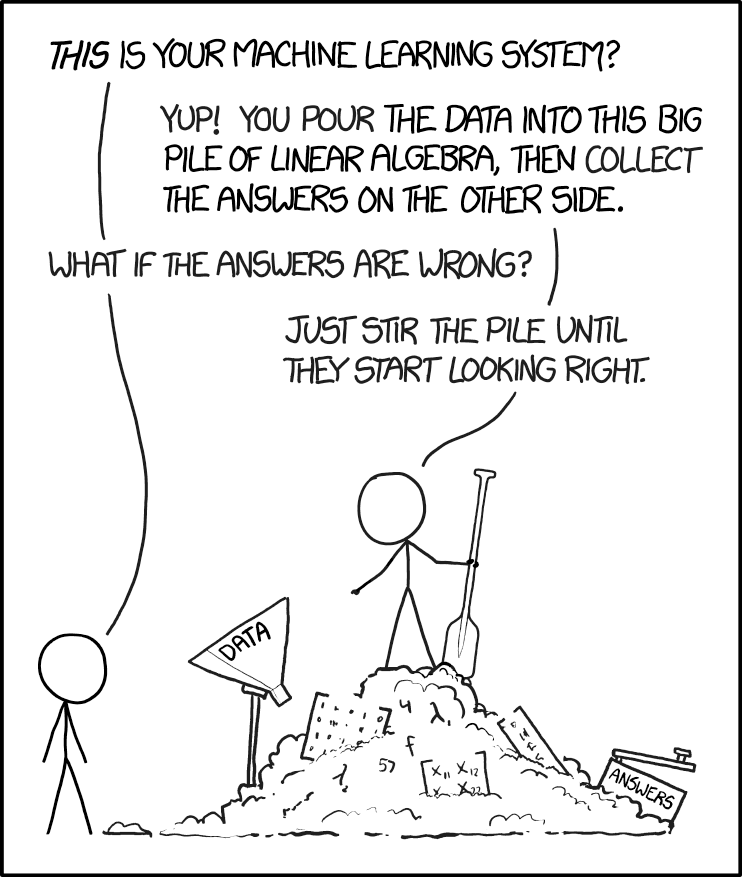
\includegraphics[width=\linewidth]{./gfx/xkcd-machineLearning}
%
\column{.5\linewidth}
\begin{Large}
	Machine Learning
	\vspace{12pt}
\end{Large}
%
\begin{center}
	\emph{The pile gets soaked with data and starts to get mushy over time, so it's technically recurrent.}
\end{center}
\begin{center}
	Source: \url{https://xkcd.com/1838/}
\end{center}
\end{columns}
%
\end{frame}

% =========================================================================== %

\begin{frame}{Definition: Machine Learning}
%
\begin{columns}[T]
\column{.4\linewidth}
\begin{itemize}
\item Humans often think of \emph{learning} as absorbing information
\item Computers can do that with ease
\item We mean learning to \emph{use} data
\item (Somewhat exaggerated: \emph{understand} data)
\item[\Thus] Need (something like) self-modifying code!
\item In particular: We'll do \emph{Deep Learning}.
\end{itemize}
%
\column{.6\linewidth}

\includegraphics[width=\linewidth]{./gfx/ML-meme}
\begin{center}
	\small
	\emph{Nope.}
\end{center}
\end{columns}
%
\end{frame}

% =========================================================================== %

\begin{frame}{Recap: What Computers are Good At}
%
\begin{itemize}
\item Name \emph{Computers} -- basic arithmetics
\item Treating numerical data
\item Handle a lot of data
\item[\Thus] Transform data into (or understand as) numbers
	\begin{itemize}
	\item Example: \emph{Is this red or white wine?} \thus binary answer \thus 1 or 0
	\item Example: Input data is an image
		\begin{itemize}
		\item Already numerical data!
		\item Ordered list of brightness information
		\item One (three) number(s) per pixel (depending on whether you use B/W or colour images)
		\end{itemize}
	\end{itemize}
\item[\Thus] Design algorithm such that (potentially a lot of) numbers describe the \enquote{thought process}
\end{itemize}
%
\end{frame}

% =========================================================================== %

\begin{frame}
%
\begin{columns}[T]
\column{.4\linewidth}
\begin{Large}
	{Image Classification}
	\vspace{12pt}
\end{Large}
%
\begin{itemize}
\item Goal: Take equally sized B/W pictures of hand written digits
\item Make the computer find out whether it is a 0, 1, ..., 9
\item Realize: Input data already in numerical form: 28x28 = 784 floating point values
\item 0: black; 1: white; 0.5: medium grey
\item Desired Output: Probability of picture showing a 0, 1, ..., 9
\item[\Thus] Input Vector \thus Output Vector
\end{itemize}
%
\column{.6\linewidth}
	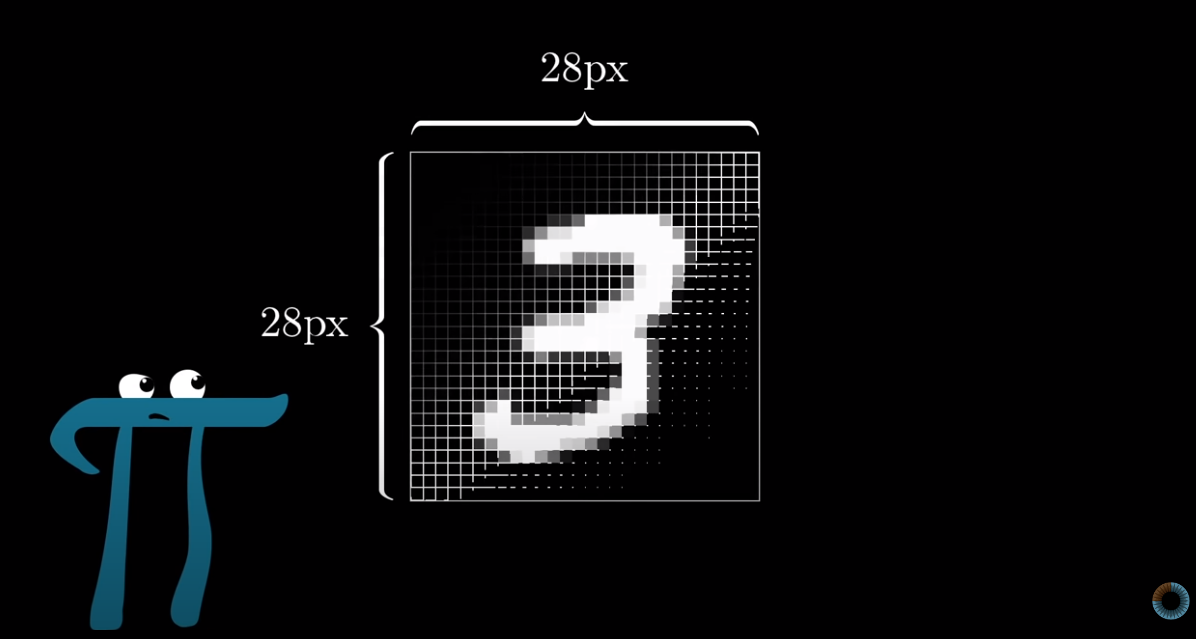
\includegraphics[width=\linewidth]{./gfx/3b1b-raster}
	\scriptsize
	Image ripped off this video:	\url{https://www.youtube.com/watch?v=aircAruvnKk}
	
	\vspace{3pt}
	3Blue1Brown does a terrific job giving intuitive understanding for abstract maths. Go check out his content. I wish I had known this channel in my first term.
\end{columns}
%
\end{frame}

% =========================================================================== %

\begin{frame}{Machine Learning as Matrix Operations}
%
\begin{itemize}
\item Possible approach: weighted, biased sums
\item $y_i$: Probability that picture shows digit $i$
\item $x_j$: $j^{\text{th}}$ pixel in the picture
\item $w_{ij}$: Weight of the $j^{\text{th}}$ pixel for the digit $i$
\item $b_j$: Bias (baseline \enquote{activation})
\item Get expression:
	\[ y_i = \sum_j w_{ij} x_j + b_i \]
\item This is a matrix multiplication and vector addition! (Assembly geeks: this is a saxpy)
	\[ \vec{y} = W \vec{x} + \vec{b} \]
\item[\Thus] \enquote{Only} need to find the correct weights $w_{ij}$ and biases $b_j$!
\end{itemize}
%
\end{frame}

% =========================================================================== %

\begin{frame}
%
\begin{columns}[T]
\column{.45\linewidth}
\begin{Large}
	{Neuronal Networks}
	\vspace{12pt}
\end{Large}
%
\begin{itemize}
\item Usually: One matrix won't do
\item But: Can perform simpler tasks (like detecting straight lines or curves)
\item Concatenate several such operations
\item[\Thus] \enquote{Hidden Layers}
\item[\Thus] Neuronal \emph{Networks}, \emph{Deep} Learning
\item Structures can become arbitrarily complex
	\begin{itemize}
	\item Parallel branches in the network
	\item Convolutions and other matrix operations
	\end{itemize}
\end{itemize}
%
\column{.55\linewidth}
	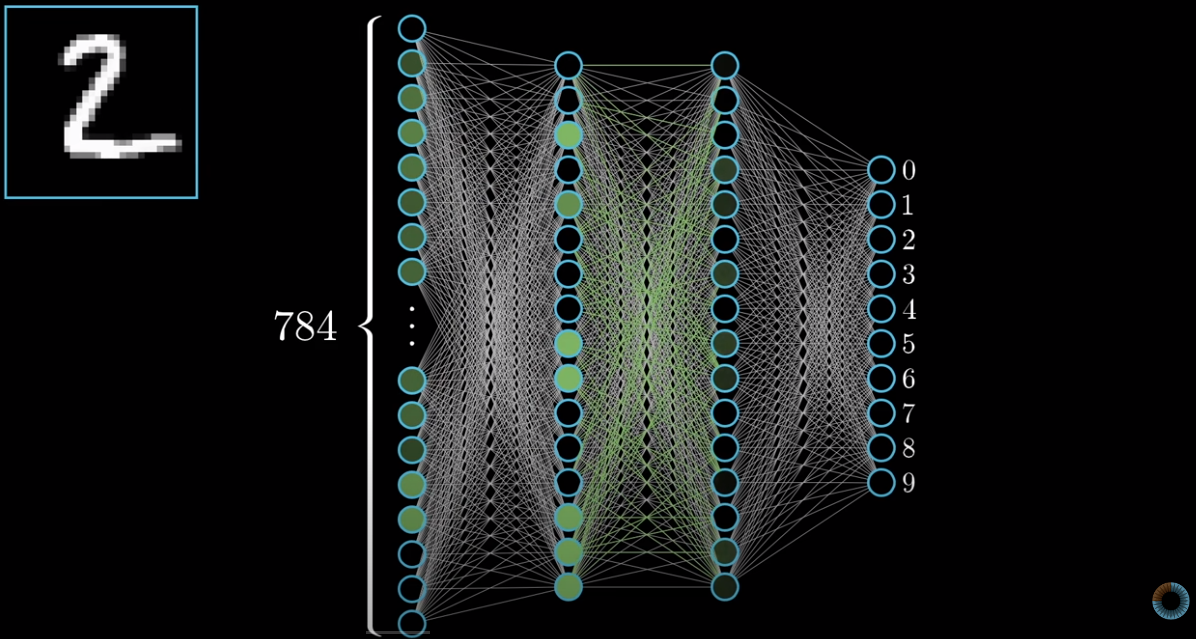
\includegraphics[width=\linewidth]{./gfx/3b1b-network}
	\scriptsize
	Samve video as before.
	
	\vspace{3pt}
	Really, these videos are just plain awesome. I wondered whether or not to simply show you his playlist on neuronal networks, as they pretty much fill one lecture.
	But there's no coding in his videos, so I figured I should actually do my job.
	
	\vspace{3pt}
	Entire Playlist:
	\url{https://www.youtube.com/playlist?list=PLZHQObOWTQDNU6R1_67000Dx_ZCJB-3pi}
\end{columns}
\vspace{6pt}
Common property: Learned data can be represented by (tens of thousands of) numbers!
%
\end{frame}

% =========================================================================== %

\begin{frame}{Additional Component: Activation Function}
%
\begin{columns}[T]
\column{.5\linewidth}
\begin{itemize}
\item So far: Chain (Network) of matrix operations
	\begin{itemize}
	\item $\vec{x}^{(0)} \to \vec{x}^{(1)} = W^{(0)} \vec{x}^{(0)} + \vec{b}^{(0)}$
	\item $\vec{x}^{(1)} \to \vec{x}^{(2)} = W^{(1)} \vec{x}^{(1)} + \vec{b}^{(1)}$
	\item ...
	\end{itemize}
\item \emph{Compositions of linear operations are again linear operations.}
\item[\Thus] This alone could be expressed in a single operation
\item Introduce a \emph{nonlinear} activation function:
\item $\vec{x}^{(l)} \to \vec{x}^{(l + 1)} = {\color{blue} f \Big(} W^{(l)} \vec{x}^{(l)} + \vec{b}^{(l)} {\color{blue} \Big)}$ 
\end{itemize}
%
\column{.5\linewidth}
	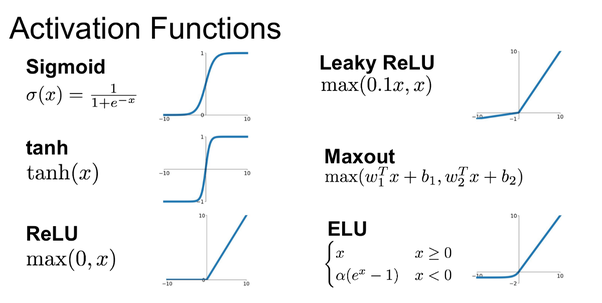
\includegraphics[width=\linewidth]{./gfx/activationFuncs}
	{\scriptsize Source:}
	{\tiny \url{https://www.quora.com/What-makes-ReLU-so-much-better-than-Linear-Activation-As-half-of-them-are-exactly-the-same}}
%
\begin{itemize}
\item ReLU: Fast to compute
\item Sigmoid: Limits output to range $(0, 1)$
\end{itemize}
\end{columns}
%
\end{frame}

% =========================================================================== %

\begin{frame}{The Main Problem Now: Learning}
%
\begin{center}
	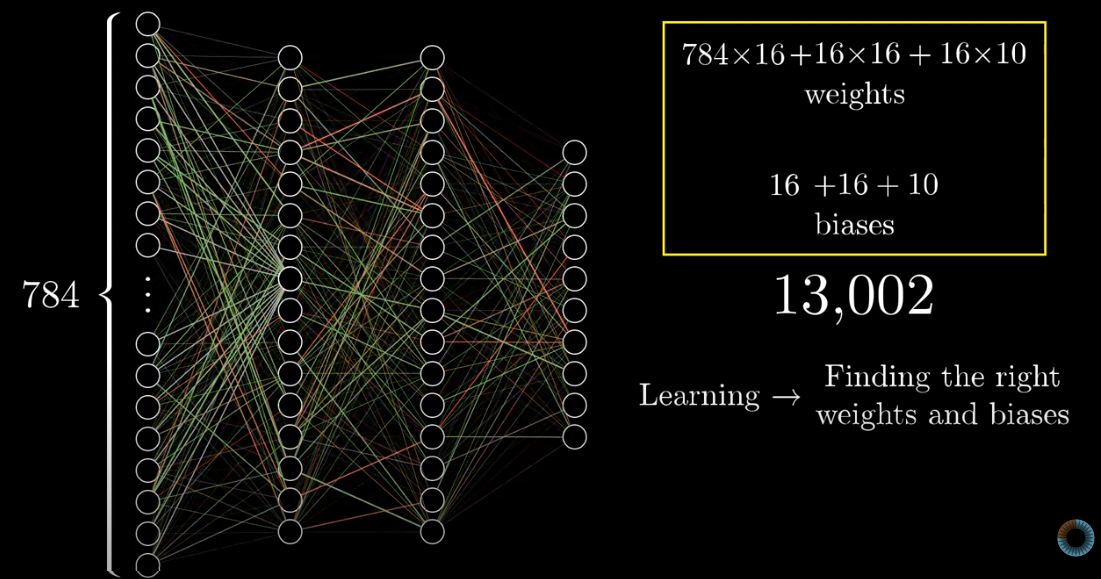
\includegraphics[width=.7\linewidth]{./gfx/3b1b-network-size}\\
	{\tiny (Guess where this is from)}
	
	\Thus \emph{But how?}
\end{center}
%
\end{frame}

% =========================================================================== %

\begin{frame}{Training}
%
\begin{itemize}
\item Start with \emph{random} weights and biases
\item Get \emph{classified} example data
	\begin{itemize}
	\item[\Thus] E.\;g. pictures with correct \enquote{label}
	\end{itemize}
\item Define a \emph{Cost Function}
	\begin{itemize}
	\item \enquote{Distance from desired result}
	\item Often: \emph{Square of Euclidian Norm}: Sum of squared differences
		\[
			\text{cost}(\vec{y}^{\text{network}}, \vec{y}^{\text{label}})
			=
			\sum_i
				\qty(
					y_i^{\text{network}} - y_i^{\text{label}}
				)^2
		\]
	\end{itemize}
\item Split into training data and test data
\item Average over all data points (\eg all images) in the training set
\item Minimize cost function by altering weights and biases
\end{itemize}
%
\end{frame}

% =========================================================================== %

\begin{frame}
%
\begin{columns}[T]
\column{.6\linewidth}
	\begin{Large}
		{A Simpler Example}
	\end{Large}
	%
	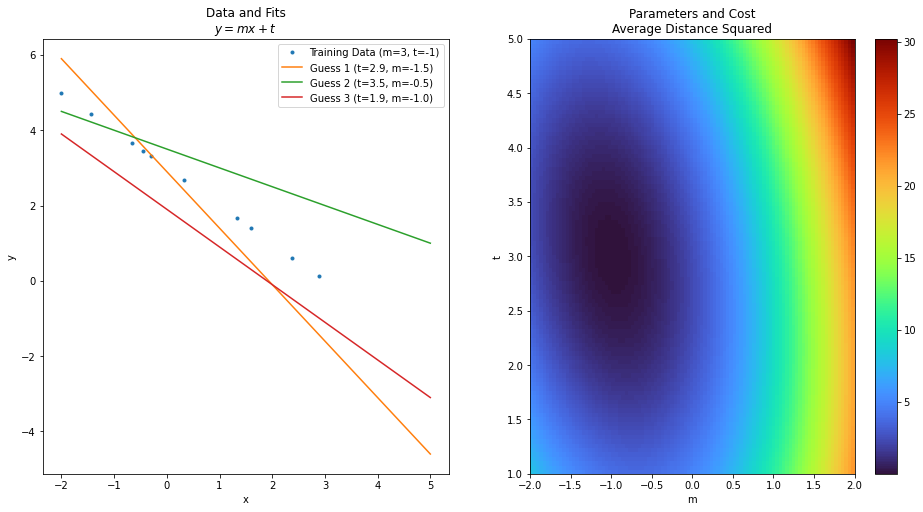
\includegraphics[width=\linewidth]{./gfx/costMap}
	%
	\begin{itemize}
	\item[\Thus] This is how SciPy's \texttt{curve\_fit} works!
	\end{itemize}
%
\column{.4\linewidth}
	\begin{itemize}
	\item X-Coordinate \textasciitilde~Image
	\item Y-Coordinate \textasciitilde~Number
	\item Parameters $m, t$ \textasciitilde~Weights and Biases
	\item Coloured lines \textasciitilde~Output of a NN
	\item Brute Force: Possible, but extremely expensive (13,002 dimensional space to explore!)
	\item Difference between \enquote{adjacent} points in cost map \textasciitilde~Gradient
	\item Steepest / gradient descent!
	\end{itemize}
\end{columns}
%
\begin{center}
\small
\emph{Note how the estimate of the NN's quality depends on the sample data! Orange line is a near-perfect fit for three points. Too few points or clustered points can give very bad results!} 
\end{center}
%
\end{frame}

% =========================================================================== %

\begin{frame}{Starting Point Dependency}
%
\begin{columns}[T]
\column{.7\linewidth}
	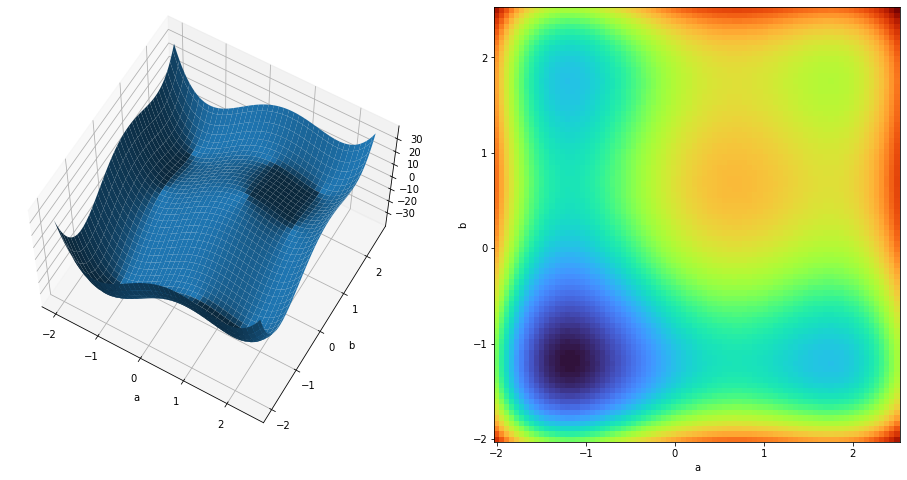
\includegraphics[width=\linewidth]{./gfx/localMins}
%
\column{.3\linewidth}
	\begin{itemize}
	\item Method of steepest descent only finds local minima!
	\item Depends on starting point
	\item[\Thus] Machine Learning Approach needs good Training Data
	\item[\Thus] Randomness always a factor
	\end{itemize}
\end{columns}
%
\end{frame}

% =========================================================================== %

\begin{frame}{Recap: Gradient Descent in Context of Machine Learning}
%
\begin{itemize}
\item We want to find the optimum weights and biases ...
\item ... to get close to the desired output ...
\item ... and evaluate the success by a cost function.
\item For the optimization we use the gradient descent method ...
\item ... which finds the weights with the highest impact (steepest slope) on the cost landscape.
\item We find a \emph{local} minimum for each single training data point ...
\item ... and hope to find the \emph{global} minimum by training with multiple data points
\end{itemize}
%
\end{frame}

% =========================================================================== %

\begin{frame}{Training Epochs and Batches}
%
\begin{itemize}
\item Training Data: \textasciitilde~10,000 data points
\item Run NN for each of the Training Data points, get changes to weights and biases, do over and over again
\item[\Thus] EXTREMELY costly
	\begin{itemize}
	\item Theory was worked out in the 1980s, but only now we have machines with sufficient power
	\item Parallelization with GPU computing
	\item Still: Takes too long
	\end{itemize}
\item Instead: Work on reduced training data subset \Thus Batches
\item Shuffle batches and repeat process \Thus Epochs
	\begin{itemize}
	\item Important to shuffle!
	\item NN could learn the order of results rather than their characteristics
	\end{itemize}
\item[\Thus] Find sweet spot of batch size and epoch count
\end{itemize}
%
\end{frame}

% =========================================================================== %

\begin{frame}{Testing}
%
\begin{itemize}
\item Once the gradient method has found an optimum for the 13,002 parameters:
\item Test with new data
	\begin{itemize}
	\item Remember: we split our source into training data and test data
	\item Reasons:
		\begin{itemize}
		\item Measure of quality
		\item Problem of overfitting
		\end{itemize}
	\item State of the art is 99.8\%
	\end{itemize}
\item Tinker with the NN properties if the success rate is not good enough
	\vspace{-6pt}
	\begin{columns}[T]
	\column{.4\linewidth}
		\begin{itemize}
		\item Learning Process
			\begin{itemize}
			\item Data Preprocessing
			\item Batch size
			\item Number of epochs
			\end{itemize}
		\end{itemize}
	%
	\column{.4\linewidth}
		\begin{itemize}
		\item NN design
			\begin{itemize}
			\item Numer of neurons in a layer
			\item Number of hidden layers
			\item Kind of layers
			\end{itemize}
		\end{itemize}
	\end{columns}
	
\end{itemize}
%
\end{frame}

% =========================================================================== %

\begin{frame}{Interpretation of the network}
%
\begin{columns}[T]
\column{.7\linewidth}
	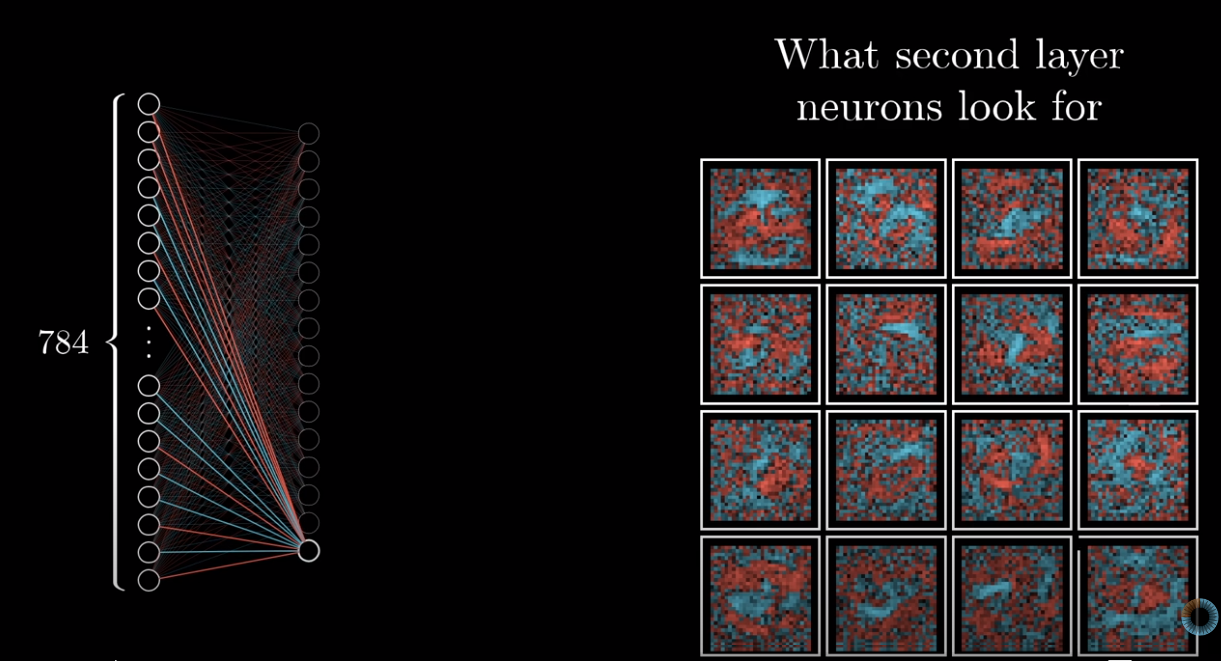
\includegraphics[width=\linewidth]{./gfx/3b1b-activation}
%
\column{.3\linewidth}
	\begin{itemize}
	\item Possible to visualize what neurons look for
	\item Hardly possible to make sense of
	\item NNs work, but make no sense of their input
	\item Feed it a picture of a cat. It might say with high confidence that it shows a 5.
	\end{itemize}
\end{columns}
%
\vspace{12pt}
{
	\scriptsize
	Image Source: \url{https://www.youtube.com/watch?v=IHZwWFHWa-w}\\
	(Again: 3Blue1Brown, Series on Machine Learning, Part 2)
}
\end{frame}

% =========================================================================== %

\begin{frame}{Network Design}
%
\begin{itemize}
\item How many layers? How many neurons per layer? What kinds of operations?
\item[\Thus] Science in its own right, almost a form of art
\item Various lectures on machine learning
\item Some Links:
	\begin{itemize}
	\item \url{https://www.datacamp.com/community/tutorials/deep-learning-python}
	\item \url{https://www.kaggle.com/learn/intro-to-machine-learning}
	\item \url{https://www.tutorialspoint.com/machine_learning_with_python/machine_learning_with_python_tutorial.pdf}
	\item \url{https://medium.com/tensorflow/mit-deep-learning-basics-introduction-and-overview-with-tensorflow-355bcd26baf0}
	\item \url{https://youtu.be/qFJeN9V1ZsI}
	\end{itemize}
\end{itemize}
%
\end{frame}

% =========================================================================== %

\begin{frame}{Implementation Time!}
%
\begin{hintbox}[Good News]
All of the logic we've just learned is implemented ready-to-use in not only one but a number of packages. For example, there's...
\begin{itemize}
\item TensorFlow (Google)
\item PyTorch (Facebook)
\item CNTK (Microsoft)
\item PlaidML (Intel)
\item Theano (University of Montreal)
\end{itemize}

\emph{Keras} is built on top of TensorFlow (it used to interface all of the above). It is a frontend (\ie a set of routines that are easy to use without understanding all the details of the underlying framework) and makes the entire Deep Learning formalism surprisingly easy to use.
\end{hintbox}
%
\end{frame}

% =========================================================================== %

\begin{frame}[fragile]{Installation}
%
\begin{cmdbox}[Installation: Anaconda]
\begin{minted}[linenos, fontsize=\scriptsize]{text}
conda install -c conda-forge keras
conda install -c conda-forge scikit-learn
\end{minted}
\end{cmdbox}
%
\begin{cmdbox}[Installation: PIP]
\begin{minted}[linenos, fontsize=\scriptsize]{text}
pip3 install keras
pip3 install -U scikit-learn
\end{minted}
\end{cmdbox}
%
\begin{hintbox}[No \texttt{sudo}]
Linux Users: don't install keras as root! \texttt{pip3} maintains separate environments, and \texttt{sudo} causes the installation to go into a different environment than the one you're most likely to use.
\end{hintbox}
%
\end{frame}

% =========================================================================== %

\begin{frame}{Code Scheme}
%
\begin{columns}[T]
\column{.55\linewidth}
	\begin{itemize}
	\item Import Modules
		\begin{itemize}
		\item \inPy{from keras.models import Sequential}\\
			\enquote{The NN}
		\item \inPy{from keras.layers import Dense}\\
			Layer (fully connected)
		\end{itemize}
	\item Load and label data
		\begin{itemize}
		\item Usually Notation:
		\item \texttt{X} -- input data
		\item \texttt{y}: output
		\end{itemize}
	\item Define the model
		\begin{itemize}
		\item \inPy{model = Sequential()}
		\item \inPy{model.add( Dense(...) )}\\
			Layers of the NN
		\end{itemize}
	\end{itemize}
%
\column{.55\linewidth}
	\begin{itemize}
	\item Compile the model
		\begin{itemize}
		\item \inPy{model.compile( ... )}
		\item Massive speedup by not running in Python
		\item May use your GraphicsCard
		\end{itemize}
	\item Fit the model
		\begin{itemize}
		\item \inPy{model.fit( ... )}
		\item Automatically finds all the parameters that minimize the loss function
		\end{itemize}
	\item Evaluate
		\begin{itemize}
		\item \inPy{loss, acc = model.evaluate(X, y)}
		\end{itemize}
	\item Use the modell
		\begin{itemize}
		\item \inPy{y_pred = model.predict(X_test)}
		\end{itemize}
	\end{itemize}
\end{columns}
%
\end{frame}

% =========================================================================== %

\begin{frame}{Code}
%
\begin{center}
	Files \texttt{016-classifyWine.py} and \texttt{classifyWine-Output.txt}
\end{center}
%
\end{frame}

% =========================================================================== %

\begin{frame}{Final Remarks}
%
\begin{itemize}
\item Deep Learning is not only good for classification, but can do all sorts of things
	\begin{itemize}
	\item Anything that converts [available numbers] into [useful numbers]
	\item AI text generation!
	\item Still, classification probably most useful
	\end{itemize}
\item Deep Learning is only \emph{one paradigm} of AI
	\begin{itemize}
	\item Support Vector Machines
	\item Cluster Analysis
	\item Principal Component Analysis
	\item ...
	\end{itemize}
\item Overfitting is a huge problem
	\begin{itemize}
	\item Perfect results on the training data does not imply practical usability
	\item NN might accidentally pick up on hidden features in the training data
	\end{itemize}
\item GIGO principle:
	\begin{itemize}
	\item Garbage in, garbage out!
	\end{itemize}
\end{itemize}
%
\end{frame}
\end{document}

% MAREI!!
% whom do I give credit? Where?